\chapter{The ``Quantum Eraser''}

\chapterprecis{Optics Practicum 4} 

\makeoddhead{myheadings}{\emph{Third Photon Practicum}}{}{\thepage}
\makeevenhead{myheadings}{\thepage}{}{\emph{The ``Quantum Eraser''}}

\section*{Introduction}

In section 3 of "The Principles of Quantum Mechanics," as we've already seen, Dirac uses the example of the interference of photons as an example of his principle of "superposition," here applied not only to the states of polarization of photons (which may or may not pass through a linear polarizer), but also to their "translational states," that is, to the multiple paths they are somehow inhabiting, according to the description Dirac says quantum mechanics provides, even of what is unobservable. Having demonstrated that even single photons may produce an interference pattern, we now turn to Dirac's further development of this idea. He writes:
\begin{quote}
Let us consider now what happens when we determine the energy in one of the components [the spatially separated beams within the interferometer]. The result of such a determination must be either the whole photon or nothing at all. Thus the photon must change suddenly from being partly in one beam and partly in the other to being entirely in one of the beams. This sudden change is due to the disturbance in the translational state of the photon which the observation necessarily makes [\,\ldots]. Our description of the photon allows us to infer that, after such an energy measurement, it would not be possible to bring about any interference effects between the two components. So long as the photon is partly in one beam and partly in the other, interference can occur when the two beams are superposed, but this possibility disappears when the photon is forced entirely into one of the beams by an observation. 
\end{quote}
We will do our best to realize this thought-experiment, though we cannot reproduce it exactly.\footnote{One version of such an experiment that is closer to Dirac's description is reported in Walborn, Terra Cunha, Pádua, and Monken, "Double-slit quantum eraser," \emph{Phys.\ Rev.\ A} \textbf{65} 033818 (2002).} As in the previous practicum, here we will send one of our beams of down-converted light through an interferometer.  Now, however, in each leg of the interferometer there will be a half-wave plate (see Figure 1).  Recall from the polarization practicum that half-wave plates rotate the polarization of the light by twice the difference in angle between the polarization of the light and the angle of the half-wave plate. The photons that enter the interferometer are vertically polarized.  Both half-wave plates should be set at zero degrees at the beginning of the practicum, so that at first they are not changing the angle of polarization.

\section*{Practicum}

Verify that the setup, with the waveplates included and set to vertical, gives the characteristic sinusoidal interference pattern as in the single photon interference practicum.  Now, turn one of the half-wave plates to 45 degrees.  This will rotate the polarization of the photon in that leg of the interferometer by 90 degrees.  Verify that the interference pattern disappears.

Dirac says that the detection of the energy of a photon in an interferometer, which would decisively indicate that the photon is in the path where its energy is measured, will make it impossible to ''bring about any interference effects between the two components.'' It appears that changing the polarization of the photons that go through one of the legs of the interferometer has a similar effect.  Dirac's thought-experiment invites us to think of changing the polarization of the photons in one of the paths of the interferometer by $90^\circ$ as equivalent to making an "observation." We do not, in fact, have anything in our apparatus that would detect the polarization of the photon coming through the interferometer, though such apparatus is certainly available to us.  But somehow the mere possibility of being able to detect which path the photon took through the interferometer seems to produce effects equivalent to those Dirac says would result from actually making an observation.

Now, as it has become common to say, we will "erase" the "which-path" information by putting a linear polarizer turned to $45^\circ$ in front of the detector, and will thereby allow the interference effects to reappear, perhaps surprisingly. Some find it significant that individual photons do not encounter the linear polarizer in front of the detector until \emph{after} they have already traversed the interferometer. Some think it important to note that, relative to the $45^\circ$ linear polarizer, the $0^\circ$ and $90^\circ$ components of the incoming light are equally passable, and come to be polarized in the same direction.   However matters may stand with these and similar sorts of considerations, it is worthwhile to trace each possible path of the photon through the interferometer and determine under which circumstances (i.e., which settings of the waveplates and polarizer) the two paths in the interferometer are in principle distinguishable.  You can test your hypotheses by trying other arrangements of the various optical elements and seeing what results you get.

%Insert Figure 1.
\begin{figure}[h]
  \centering
    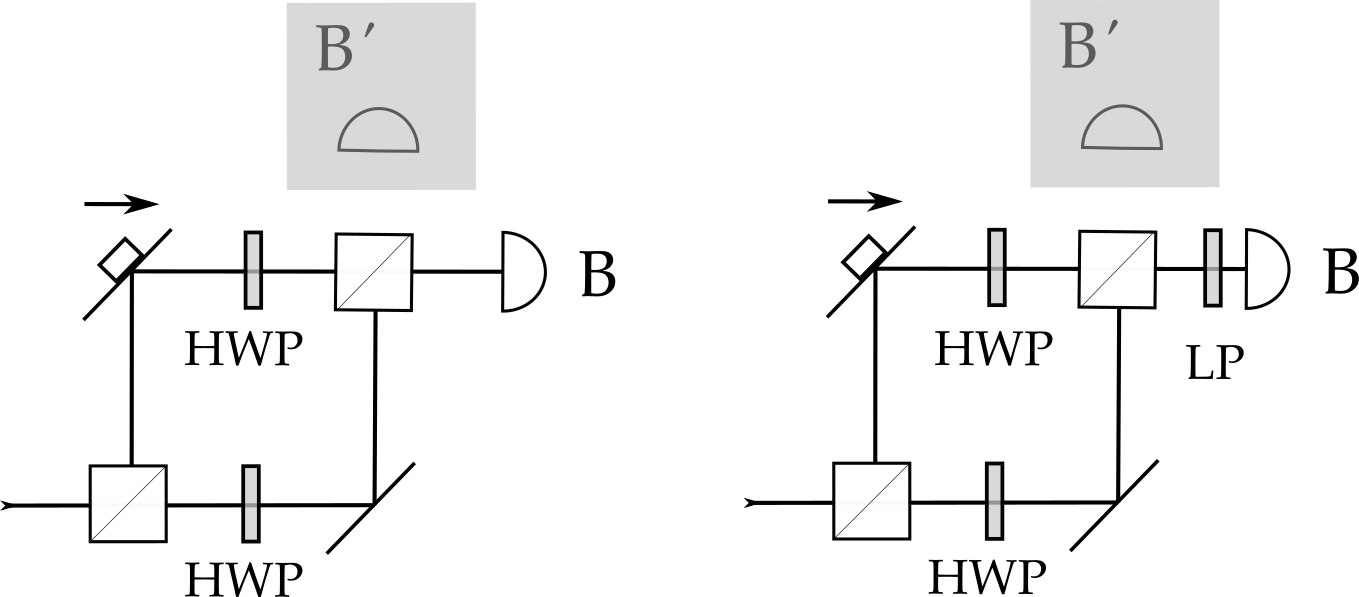
\includegraphics[width=4.53in,height=1.99in]{images/15_quantum-eraser/complete.png}
    \captionsetup{width=.75\textwidth}
    \caption*{Figure 1 --- \emph{Experimental setup for the ``quantum eraser,'' showing the two stages of the 
    demonstration. An optional second detector can be set up at $B'$ if desired after the main demonstration is complete.}}
\end{figure}
